%% mcl.tex
%% Author: Leighton Pritchard
%% Copyright: James Hutton Institute
%% An outline of using MCL for orthologue finding

% 
\begin{frame}
  \frametitle{MCL
    \footnote{\tiny{Enright \textit{et al.} (2002) \textit{Nucl. Acids Res.} \href{http://dx.doi.org/10.1093/nar/30.7.1575}{doi:10.1093/nar/30.7.1575
    }}}
  }
  \begin{itemize}
    \item MCL constructs a network (\textit{graph}) from all-against-all BLAST results
    \item \textcolor{hutton_green}{Matrix operations (\textit{expansion}, \textit{inflation}) are applied}
    \item \textcolor{hutton_blue}{Expansion, inflation iterated until the network converges}
  \end{itemize}
  \begin{center}
      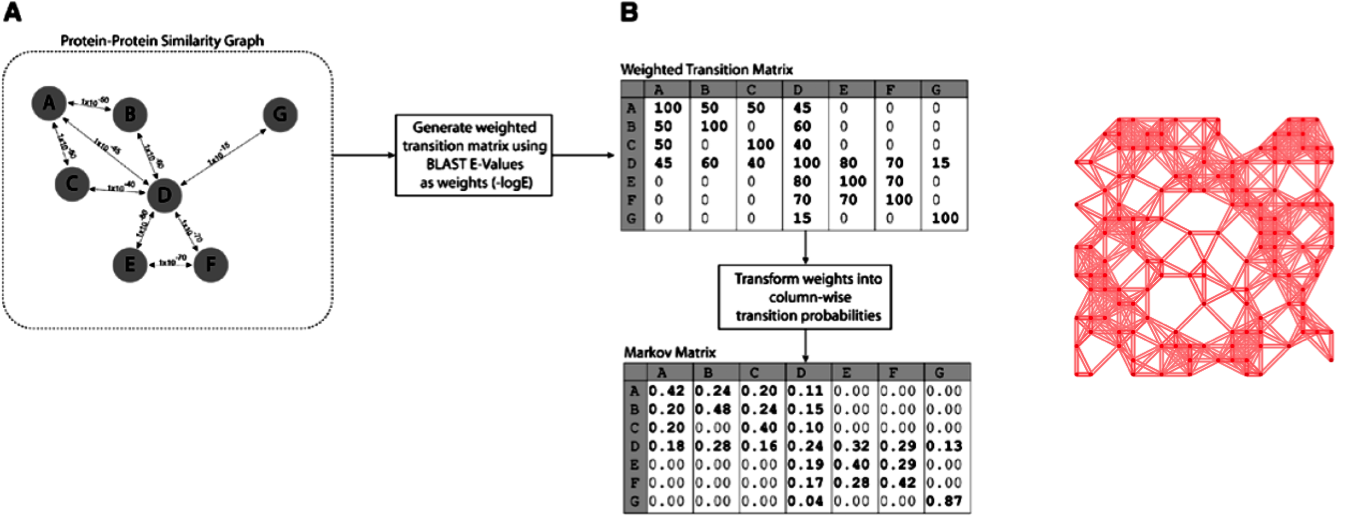
\includegraphics[width=1\textwidth]{images/mcl_intro}
  \end{center}
\end{frame}

% 
\begin{frame}
  \frametitle{MCL
    \footnote{\tiny{Enright \textit{et al.} (2002) \textit{Nucl. Acids Res.} \href{http://dx.doi.org/10.1093/nar/30.7.1575}{doi:10.1093/nar/30.7.1575
    }}}
  }  
  \begin{center}
      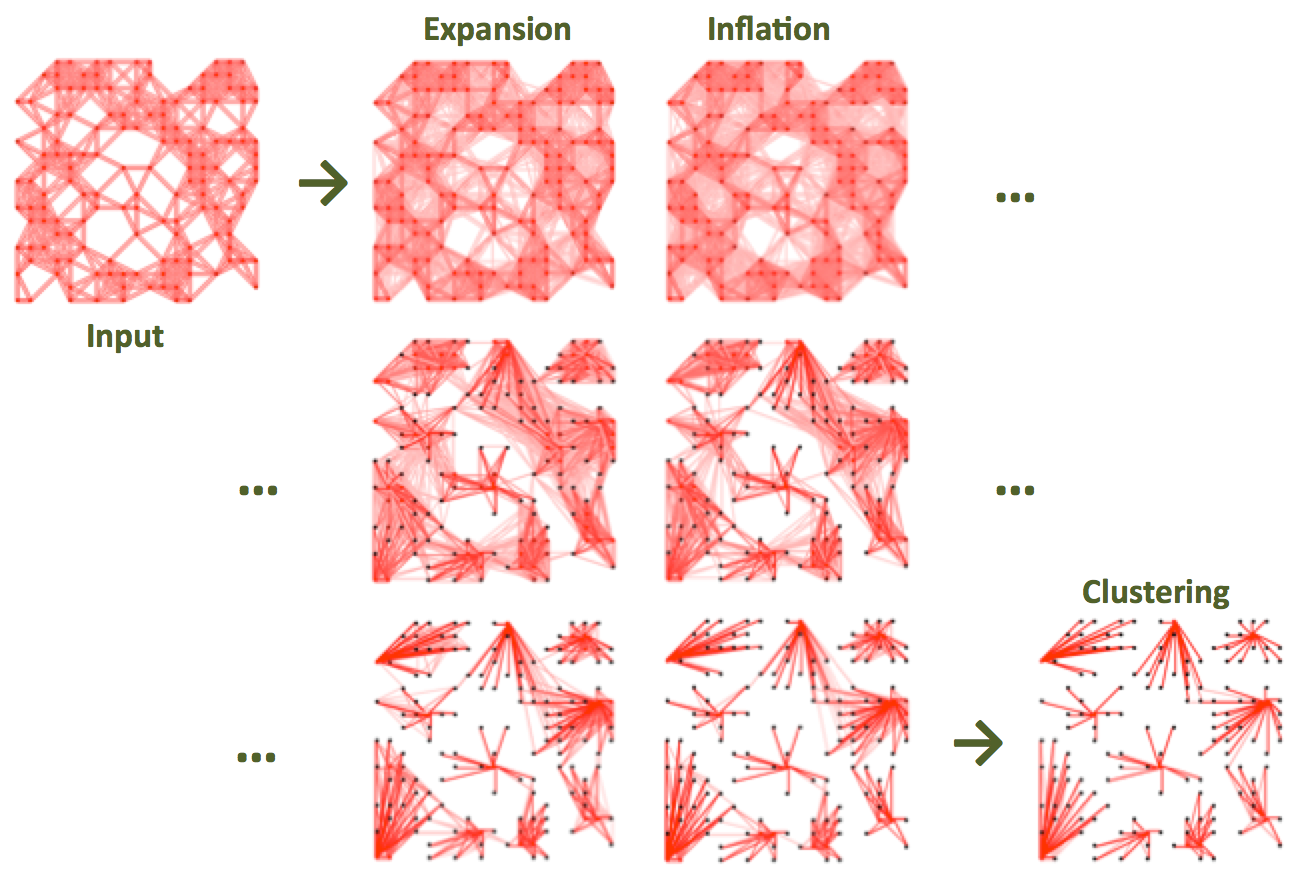
\includegraphics[width=1\textwidth]{images/mcl_method}
  \end{center}
\end{frame}

% 
\begin{frame}
  \frametitle{OrthoMCL
    \footnote{\tiny{Li \textit{et al.} (2003) \textit{Genome Res.} \href{http://dx.doi.org/10.1101/gr.1224503
}{doi:10.1101/gr.1224503
    }}}
    \footnote{\tiny \href{http://orthomcl.org/orthomcl/}{http://orthomcl.org/orthomcl/}
    }
  }
  \begin{itemize}
    \item Defines potential inparalogue, orthologue and co-orthologue pairs, \textcolor{red}{using RBBH}
    \item \textcolor{hutton_green}{Applies MCL to cluster these pairs of sequences}
    \item \textcolor{hutton_blue}{Output clusters include both orthologues and paralogues}
  \end{itemize}  
  \begin{center}
      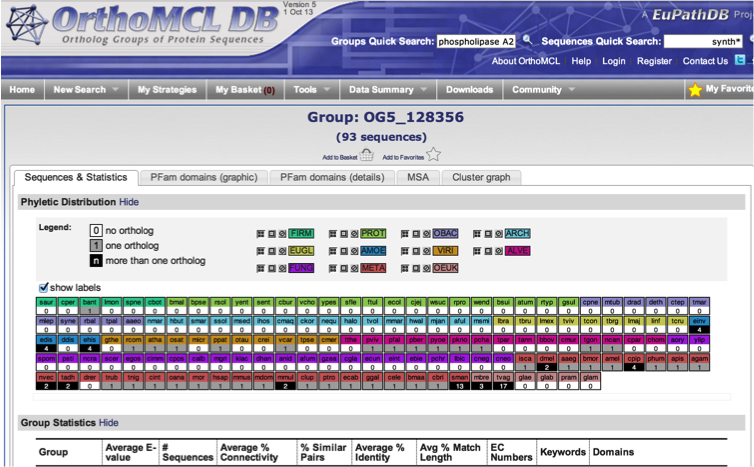
\includegraphics[width=0.7\textwidth]{images/orthomcl}
  \end{center}
\end{frame}

%
\begin{frame}
  \frametitle{Finding ``Orthologues'': MCL}
  \Large{
    \textcolor{hutton_blue}{
      \textbf{
      EXERCISE 9: \\
      {\small \href{https://github.com/widdowquinn/Teaching-2015-03-17-UoD_compgenvis/blob/master/exercises/mcl_orthologues/ex09a_mcl_orthologues.md}{\texttt{mcl\_orthologues/ex\_09a\_mcl\_orthologues.md}} \\
      \texttt{mcl\_orthologues/ex09b\_mcl\_orthologues.ipynb}}
      }
    }
  }
\end{frame}